%%%%%%%%%%%%%%%%%%%%%%%%%%%%%%%%%%%%%%%%%%%%%%%%%%%%%%%%%%%%%%%%%%%%%%%%%%%%%%%%%%%%%%%%%%%%%%
%%%%%%%%%%%%%%%%%%%%%%%%%%%%%%%%%%%%%%%%%%%%%%%%%%%%%%%%%%%%%%%%%%%%%%%%%%%%%%%%%%%%%%%%%%%%%%
%%%%%%%%%%% Estimators
%%%%%%%%%%%%%%%%%%%%%%%%%%%%%%%%%%%%%%%%%%%%%%%%%%%%%%%%%%%%%%%%%%%%%%%%%%%%%%%%%%%%%%%%%%%%%%
%%%%%%%%%%%%%%%%%%%%%%%%%%%%%%%%%%%%%%%%%%%%%%%%%%%%%%%%%%%%%%%%%%%%%%%%%%%%%%%%%%%%%%%%%%%%%%


% \cleardoublepage
\chapter{PAQ Equations}
\label{chap:equations}

This thesis studies GPU implementation of the PAQ project data-aided FIR equalizer filters.
The impulse response of the FIR equalizer filters are computed using channel and noise variance estimates based on the iNET preamble and ASM in the received signal.
%The channel and noise variance estimates are very susceptible to frequency offset.
%The frequency offset must be estimated then removed.
All the estimates are data-aided and thus require finding the preamble and the ASM in the received signal.
A preamble detector is employed to estimate the start of each iNET packet in the set.
Figure \ref{fig:estimators} shows a block diagram of the estimators in the PAQ project.
The data-aided FIR equalizer filters are then computed and the received samples are equalized.
With the received samples equalized, a detection filter is applied and the symbols are estimated using a OQPSK detector.
Figure \ref{fig:thisThesisBlock} shows a block diagram of the FIR filters and symbol detector in the PAQ project.

The estimators, detection filter and OQPSK detector will be briefly explained in Section \ref{sec:estimators}.
Section \ref{sec:equalizer_eq} will explain the equations for the FIR equalizer filters and the application of the equalizers and detection filter.

\section{Estimators}
\label{sec:estimators}
\subsection{Preamble Detection}
\label{sec:pd}
To compute data-aided equalizers, preambles in the received signal are found then used to estimate parameters.
The goal of the preamble detection step is to structure the received samples $r(n)$ into $\Lpkt$ sample packets $\mathbf{r}_\text{p}$.
Each vector of samples $\mathbf{r}_\text{p}$ has the structure shown in Figure \ref{fig:packetStructure_intro}.

Before the structuring the received samples into packets, the preambles are found using the preamble detector explained in \cite{preamble_detector}.
The preamble detector computes the function $L(n)$ for each sample in the set.
Peaks in $L(n)$ identify the locations of a preamble or the start of a packet.
The function $L(n)$ is given by
\begin{equation}
	L(n) = \sum_{m=0}^{7}
		\left[ I^2(n,m) + Q^2(n,m) \right]
	\label{eq:gpu-L-4}
\end{equation}
where
\begin{multline}
	I(n,m) \approx \sum_{\ell\in\mathcal{L}_1}r_R(\ell+32m+n)
			- \sum_{\ell\in\mathcal{L}_2}r_R(\ell+32m+n)
			+ \sum_{\ell\in\mathcal{L}_3}r_I(\ell+32m+n)
			- \sum_{\ell\in\mathcal{L}_4}r_I(\ell+32m+n)
			\\
			+ 0.7071 \left[
				\sum_{\ell\in\mathcal{L}_5}r_R(\ell+32m+n)
				- \sum_{\ell\in\mathcal{L}_6}r_R(\ell+32m+n)
			\right. \\
			\left.
				+ \sum_{\ell\in\mathcal{L}_7}r_I(\ell+32m+n)
				- \sum_{\ell\in\mathcal{L}_8}r_I(\ell+32m+n)
			\right],
	\label{eq:gpu-L-pedone-geoghegan-2}
\end{multline}
and
\begin{multline}
	Q(n,m) \approx \sum_{\ell\in\mathcal{L}_1}r_I(\ell+32m+n)
			- \sum_{\ell\in\mathcal{L}_2}r_I(\ell+32m+n)
			\\
			- \sum_{\ell\in\mathcal{L}_3}r_R(\ell+32m+n)
			+ \sum_{\ell\in\mathcal{L}_4}r_R(\ell+32m+n)
			\\
			+ 0.7071 \left[
				\sum_{\ell\in\mathcal{L}_5}r_I(\ell+32m+n)
				- \sum_{\ell\in\mathcal{L}_6}r_I(\ell+32m+n)
			\right. \\
			\left.
				- \sum_{\ell\in\mathcal{L}_7}r_R(\ell+32m+n)
				+ \sum_{\ell\in\mathcal{L}_8}r_R(\ell+32m+n)
			\right]
		\label{eq:gpu-L-pedone-geoghegan-3}
\end{multline}
with
\begin{equation}
	\begin{split}
	\mathcal{L}_1 &= \{ 0, 8, 16, 24 \}\\
	\mathcal{L}_2 &= \{ 4, 20 \}\\
	\mathcal{L}_3 &= \{ 2, 10, 14, 22 \}\\
	\mathcal{L}_4 &= \{ 6, 18, 26, 30 \}\\
	\mathcal{L}_5 &= \{ 1, 7,  9, 15, 17, 23, 25, 31 \}\\
	\mathcal{L}_6 &= \{ 3, 5, 11, 12, 13, 19, 21, 27, 28, 29 \}\\
	\mathcal{L}_7 &= \{ 1, 3,  9, 11, 12, 13, 15, 21, 23 \}\\
	\mathcal{L}_8 &= \{ 5, 7, 17, 19, 25, 27, 28, 29, 31 \}.
\end{split}
\label{eq:gpu-L-pedone-geoghegan-4}
\end{equation}
A correlation peak in $L(n)$ indicates the index $n$ is the start of a preamble.
The vector of packet samples starting at index $n$ are
\begin{equation}
\mathbf{r}_\text{p} = 
\begin{bmatrix}
r(n) \\ 
\vdots \\ 
r(n+\Lpkt-1)
\end{bmatrix}
=
\begin{bmatrix}
r_\text{p}(0) \\ 
\vdots \\ 
r_\text{p}(\Lpkt-1)
\end{bmatrix}
\end{equation}

\subsection{Frequency Offset Compensation}
\label{sec:freq_offset_comp}
The frequency offset estimator shown in Figure \ref{fig:estimators} is the estimator taken from \cite[eq. (24)]{rice2014frequency}.
With the notation adjusted slightly, the frequency offset estimate is
\begin{equation}
	\hat{\omega}_0 = \frac{1}{L_q} \arg\left\{ \sum_{n=i+2L_q}^{i+7L_q-1} r_\text{p}(n)r_\text{p}^\ast(n-L_q)\right\}
	\quad
\text{for} \;
i=1,2,3,4,5.
	\label{eq:jeff-ML-w-final3}
\end{equation}
The frequency offset is estimated for every packet or each vector of samples $\mathbf{r}_\text{p}$ in the set.
Frequency offset compensation is performed by de-rotating the received samples by $-\hat{\omega}_0$:
\begin{equation}
	r(n) = r_\text{p}(n) e^{-j\hat{\omega}_0n}.
	\label{eq:frequency_compensation}
\end{equation}
Equations \eqref{eq:jeff-ML-w-final3} and \eqref{eq:frequency_compensation} are easily implemented into GPUs. 

\subsection{Channel Estimation}
\label{sec:channel_estimation}
The channel estimator is the ML estimator taken from \cite[eq. 8]{rice-afran-saquib-cole-rhodes-moazzami:2014}.
\begin{equation}
\hat{\mathbf{h}} = \underbrace{ \left( \mathbf{X}^\dag\mathbf{X} \right)^{-1} \mathbf{X}^\dag}_{\mathbf{X}_\text{lpi}}\mathbf{r}
\end{equation}
where 
\begin{equation}
\mathbf{X} = 
		\begin{bmatrix}
		p(N_2)							& 								& 		&  			\\
		\vdots 							& p(N_2)						& 		&  			\\
		p(L_\text{p}+L_\text{ASM}-N_1)	&\vdots							& \ddots&  			\\
										& p(L_\text{p}+L_\text{ASM}-N_1)&  		& p(N_2)  	\\
		 								&  								&  		& \vdots 	\\
		 								&  	   							&  		& p(L_\text{p}+L_\text{ASM}-N_1)\\
	\end{bmatrix}
\end{equation}
is a $(L_\text{p}+L_\text{ASM}-N_1-N_2)\times(N_1+N_2+1)$ convolution matrix formed from the ideal preamble and ASM samples.
The $(N_1+N_2+1)\times(L_\text{p}+L_\text{ASM}-N_1-N_2)$ matrix $\mathbf{X}_\text{lpi}$ is the left pseudo-inverse of $\mathbf{X}$.
The ML channel estimator is the result of the matrix operation
\begin{equation}
\hat{\mathbf{h}} = \mathbf{X}_\text{lpi} \mathbf{r}.
\end{equation}
The matrix operation $\mathbf{X}_\text{lpi} \mathbf{r}$ is implemented simply and efficiently in GPUs.


\subsection{Noise Variance Estimation}
\label{sec:noise_variance_estimation}
The noise variance estimator is also taken from \cite[eq. 9]{rice-afran-saquib-cole-rhodes-moazzami:2014}
\begin{equation}
	\hat{\sigma}_w^2 = \frac{1}{2\rho} \left| \mathbf{r}-\mathbf{X}\hat{\mathbf{h}}\right|^2
	\label{eq:ML-s2-final3}
\end{equation}
where
\begin{equation}
	\rho = {\rm Trace} \left\{ \mathbf{I} -  \mathbf{X}\left(\mathbf{X}^\dag\mathbf{X}\right)^{-1}\mathbf{X}^\dag \right\}.
\end{equation}
Equation \eqref{eq:ML-s2-final3} is easily implemented into GPUs.


\subsection{Symbol-by-Symbol Detector}
\label{sec:oqpsk_detector}
Symbol-by-symbol detection comprises a detection filter and a phase lock loop (PLL) to track out the residual frequency offset.
Before the symbols are detected, the equalized samples are passed through the detection filter then down-sampled by $2$. 
The detection filter is a $L_\text{df} = 21$ sample ``numerically optimized'' SOQPSK detection filter $H_\text{NO}$ \cite[Fig. 3]{perrins:2013}.
The symbol-by-symbol detector block in Figure \ref{fig:thisThesisBlock} is a Offset Quaternary Phase Shift Keying (OQPSK) detector.
Using the simple OQPSK detector in place of a complex MLSE SOQPSK-TG detector leads to less than $1$ dB loss in detection efficency \cite{perrins:2013}.
\begin{figure}
	\centering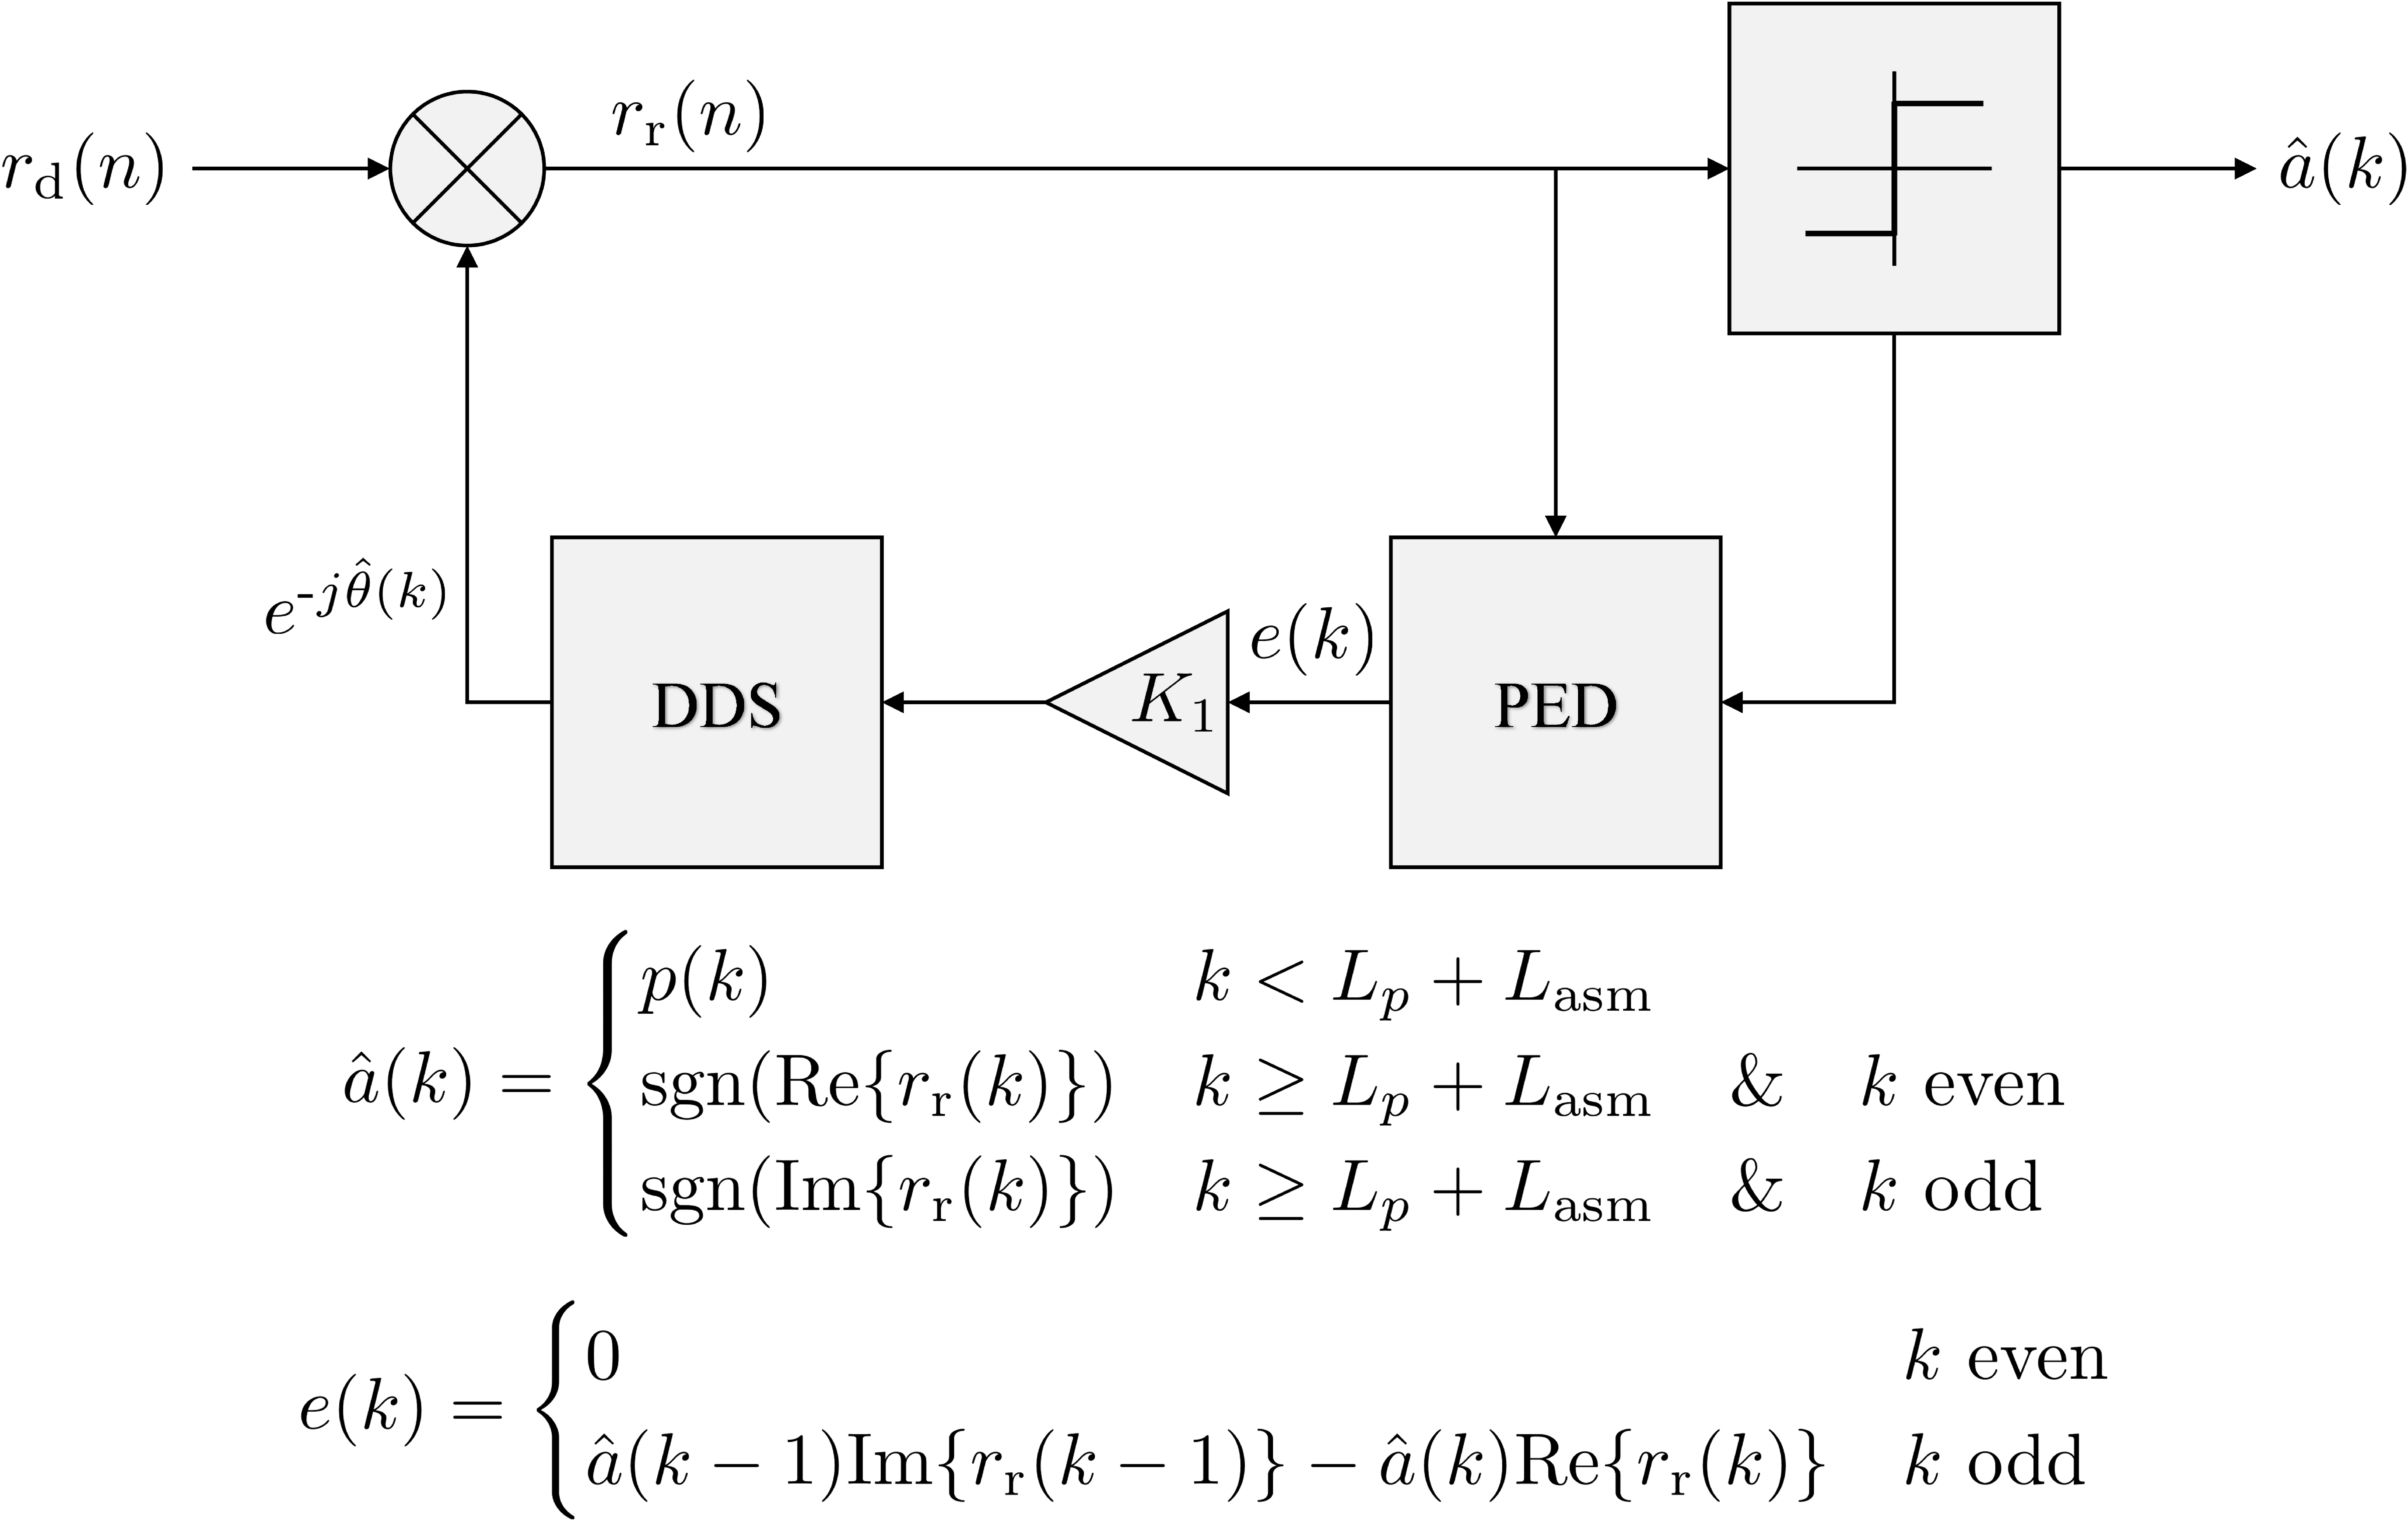
\includegraphics[width=9.11in/100*55]{figures/systemOverview/OQPSK.pdf}
	\caption{Offset Quadriture Phase Shift Keying symbol by symbol detector.}
	\label{fig:OQPSK}
\end{figure}

A Phase Lock Loop (PLL) is needed in the OQPSK detector to track out residual frequency offset.
The residual frequency offset results from a frequency offset estimation error.
While phase offset, timing offset and multipath are combated with equalizers, batched based equalizers cannot remove residual frequency offset.
The PLL tracks out the residual frequency offset using a feedback control loop.

Implementing a PLL may not seem feasible in GPUs because the feedback loop cannot be parallelized.
But the PAQ system processes $3104$ batches of data at a time by parallelizing on a packet by packet basis.
Running the PLL and detector serially through a full packet of samples is relatively fast because each iteration requires only $10$ floating point operations and a few logic decisions.


\section{Equalizers}
\label{sec:equalizer_eq}
This thesis examines that performance and GPU implementation of five FIR equalizer filters.
While the performance and GPU implementation is interesting, this thesis makes no claim of theoretically expanding understanding of equalizers.
The data-aided equalizers studied in this thesis are:
\begin{itemize}
\item zero-forcing (ZF) equalizer
\item minimum mean square Error (MMSE) equalizer
\item MMSE initialized constant modulus algorithm (CMA) equalizer
\item frequency domain equalizer one (FDE1)
\item frequency domain equalizer Two (FDE2).
\end{itemize}
The final equations for ZF and MMSE FIR equalizer filters are very similar but differ in formulation.
The equations for FDE1 and FDE2 are also very similar but differ by one subtle difference.
The CMA FIR equalizer filter is computed using a steepest decent algorithm initialized by MMSE.
More CMA iterations lead to lower BER but ZF, MMSE, FDE1 and FDE2 only require one iteration.
The equations explained in this section will be referenced heavily in Chapter \ref{chap:equalizers_in_gpus}.

\subsection{Zero-Forcing and Minimum Mean Square Error Equalizers}
\label{sec:ZFnMMSE}
The ZF and MMSE equalizers are treated together here because they have many common features.
Both equalizers are found by solving linear equations
\begin{equation}
\mathbf{A}\mathbf{c} = \mathbf{b}
\end{equation}
where $\mathbf{c}$ is a vector of desired equalizer coefficients
and the matrix $\mathbf{A}$ and vector $\mathbf{b}$ are known.
It will be shown that the only difference between ZF and MMSE lies in the matrix $\mathbf{A}$.

\subsubsection{Zero-Forcing}
\label{sec:zero-forcing}
The ZF equalizer is an FIR filter defined by the coefficients
\begin{equation}
\begin{matrix}
c_\text{ZF}(-L_1) & \cdots & c_\text{ZF}(0) & \cdots & c_\text{ZF}(L_2).
\end{matrix}
\end{equation}
The filter coefficients are the solution to the matrix vector equation \cite[eq. (311)]{PAQ-phase1}
\begin{equation}
\mathbf{c}_\text{ZF} = \big(\mathbf{H}^\dagger\mathbf{H}\big)^{-1} \mathbf{H}^\dagger \mathbf{u}_{n_0}
\label{eq:c_ZF_direct}
\end{equation}
where
\begin{equation}
\mathbf{c}_\text{ZF} = 
\begin{bmatrix}
c_\text{ZF}(-L_1) \\ \vdots \\ c_\text{ZF}(0) \\ \vdots \\ c_\text{ZF}(L_2)
\end{bmatrix},
\end{equation}
\begin{equation}
\mathbf{u}_{n_0} = \begin{bmatrix} 0 \\ \vdots \\ 0 \\ 1 \\ 0 \\ \vdots \\ 0 \end{bmatrix}
	\begin{matrix*}[l] \left. \vphantom{\begin{matrix} 0 \\ \vdots \\ 0 \end{matrix}} \right\}
		\text{$n_0-1$ zeros}
		\\ \\
		\left. \vphantom{\begin{matrix} 0 \\ \vdots \\ 0 \end{matrix}} \right\}
		\text{$N_1+N_2+L_1+L_2-n_0+1$ zeros}
		\end{matrix*},
		\label{eq:un0_ZF}
\end{equation}
where $n_0 = N_1+L_1+1$ and
\begin{equation} 
\mathbf{H} = 
		\begin{bmatrix}
		\hat{h}(-N_1)		&  				& 		 	&  					\\
		\hat{h}(-N_1+1) 	& \hat{h}(-N_1)	& 		 	&  					\\
		\vdots	 			& \vdots		& \ddots 	&  					\\
		\hat{h}(N_2)		& \hat{h}(N_2-1)&  			& \hat{h}(-N_1)  	\\
		 					& \hat{h}(N_2) 	&  			& \hat{h}(-N_1+1) 	\\
		 					&  	   			&  			& \vdots			\\
		 					&  	   			&  			& \hat{h}(N_2)		\\
	\end{bmatrix}.
\end{equation}

Equation \eqref{eq:c_ZF_direct} can be implemented directly but there are many optimization that greatly reduce computation.
The heaviest computation is the $\mathcal{O}(n^3)$ inverse operation followed by the $\mathcal{O}(n^2)$ matrix matrix multiplies.
Rather than performing a heavy inverse, multiplying $\mathbf{H}^\dagger \mathbf{H}$ on both sides of equation \eqref{eq:c_ZF_direct} results in
\begin{align}
\mathbf{H}^\dagger\mathbf{H} \mathbf{c}_\text{ZF} &= \mathbf{H}^\dagger \mathbf{u}_{n_0} \nonumber \\
\mathbf{R}_{\hat{h}} \mathbf{c}_\text{ZF} &= \hat{\mathbf{h}}_{n_0}
\label{eq:c_ZF_solve}
\end{align}
where
\begin{equation}
\mathbf{R}_{\hat{h}} = 
\mathbf{H}^\dagger \mathbf{H} = 
		\begin{bmatrix}
		r_{\hat{h}}(0)			& r^\ast_{\hat{h}}(1)	& \cdots 	& r^\ast_{\hat{h}}(L_{eq}-1)  	\\
		r_{\hat{h}}(1) 			& r_{\hat{h}}(0)		& \cdots 	& r^\ast_{\hat{h}}(L_{eq}-2)  	\\
		\vdots	 				& \vdots				& \ddots 	&  								\\
		r_{\hat{h}}(L_{eq}-1)	& r_{\hat{h}}(L_{eq}-2)	& \cdots	& r_{\hat{h}}(0)  			
	\end{bmatrix}
	\label{eq:R_h}
\end{equation}
is the auto-correlation matrix of the channel estimate $\hat{\mathbf{h}}$
and 
\begin{equation}
\hat{\mathbf{h}}_{n_0} = \mathbf{H}^\dagger \mathbf{u}_{n_0} = 
\begin{bmatrix} \hat{h}^\ast(L_1) \\ \vdots \\ \hat{h}^\ast(0) \\ \vdots \\ \hat{h}^\ast(-L_2)  \end{bmatrix}
\label{eq:h_no}
\end{equation}
is a vector with the time reversed and conjugated channel estimate $\hat{\mathbf{h}}$ centered at $n_0$.
The channel estimate auto-correlation sequence is
\begin{equation}
r_{\hat{h}}(k) = \sum_{n=-N_1}^{N_2} \hat{h}(n) \hat{h}^\ast(n-k).
\label{eq:sample_autocorrelation}
\end{equation}
Note that the auto-correlation matrix $\mathbf{R}_{\hat{h}}$ is comprised of 
\begin{equation}
\mathbf{r}_{\hat{h}} = 
\begin{bmatrix} r_{\hat{h}}(0) \\ \vdots \\ r_{\hat{h}}(L_{ch}) \\ r_{\hat{h}}(L_{ch}+1) \\ \vdots \\ r_{\hat{h}}(L_{eq}-1)\end{bmatrix} =
\begin{bmatrix} r_{\hat{h}}(0) \\ \vdots \\ r_{\hat{h}}(L_{ch}) \\ 0 \\ \vdots \\ 0  \end{bmatrix}.
\end{equation} 
Using $\mathbf{r}_{\hat{h}}$ eliminates the need for matrix matrix multiply of $\mathbf{H}^\dagger\mathbf{H}$.
Also, $r_{\hat{h}}(k)$ only has support on $-(L_{ch}-1) \leq k \leq L_{ch}-1$ making $\mathbf{R}_{\hat{h}}$ sparse or $\%63$ zeros. NEEDS CHECKING!!!!
The sparseness of $\mathbf{R}_{\hat{h}}$ can be leveraged to reduce computation drastically.

\subsubsection{MMSE Equalizer}
The MMSE equalizer is an FIR filter defined by the coefficients
\begin{equation}
\begin{matrix}
c_\text{MMSE}(-L_1) & \cdots & c_\text{MMSE}(0) & \cdots & c_\text{MMSE}(L_2).
\end{matrix}
\end{equation}
The filter coefficients are the solution to the matrix vector equation \cite[eq. (330) and (333)]{PAQ-phase1}
\begin{equation}
\mathbf{c}_\text{MMSE} = \big[ \mathbf{G}\mathbf{G}^\dagger + 2\hat{\sigma}^2_w\mathbf{I}_{L_1+L_2+1} \big]^{-1} \mathbf{g}^\dagger
\label{eq:c_MMSE_direct}
\end{equation}
where $\mathbf{I}_{L_1+L_2+1}$ is the $(L_1+L_2+1)\times(L_1+L_2+1)$ identity matrix,
$\hat{\sigma}^2_w$ is the estimated noise variance, $\mathbf{G}$ is the $(L_1+L_2+1)\times(N_1+N_2+L_1+L_2+1)$ matrix given by
\begin{equation}
\mathbf{G} = 
		\begin{bmatrix}
		\hat{h}(N_2)		& \cdots		& \hat{h}(-N_1) 	&  				  \\
							& \hat{h}(N_2)	& \cdots 			& \hat{h}(-N_1)	  \\
				 			& 				& \ddots 			&  				& \ddots	  \\
		 					&  	   			&  					& \hat{h}(N_2)	& \cdots	& \hat{h}(-N_1)	\\
	\end{bmatrix}
\end{equation}
and $\mathbf{g}^\dagger$ is the $(L_1+L_2+1)\times1$ vector given by
\begin{equation}
\mathbf{g}^\dagger = \hat{\mathbf{h}}_{n0} = \begin{bmatrix} \hat{h}^\ast(L_1) \\ \vdots \\ \hat{h}^\ast(0) \\ \vdots \\ \hat{h}^\ast(-L_2)  \end{bmatrix}.
%\begin{bmatrix} \hat{h}(L_1) \cdots \hat{h}(-L_2) \end{bmatrix}.
\label{eq:g_dagger_h_n0}
\end{equation}

Computing $\mathbf{c}_\text{MMSE}$ can be simplified by noticing that $\mathbf{g}^\dagger = \hat{\mathbf{h}}_{n_0}$, $\mathbf{G}\mathbf{G}^\dagger = \mathbf{R}_{\hat{h}}$ in Equation \eqref{eq:R_h}.
To further simplify MMSE, twice the estimated noise variance is added down the diagonal of the channel estimate auto-correlation matrix
\begin{equation}
\mathbf{R} = 
\mathbf{R}_{\hat{h}} + 2\hat{\sigma^2_w} \mathbf{I}_{L_1+L_2+1} = 
		\begin{bmatrix}
		r_{h}(0) + 2\hat{\sigma^2_w}	& r^\ast_{h}(1)							& \cdots 	& r^\ast_{h}(L_{eq}-1)  	\\
		r_{h}(1) 						& r_{h}(0) + 2\hat{\sigma^2_w}& \cdots 	& r^\ast_{h}(L_{eq}-2)  				\\
		\vdots	 						& \vdots								& \ddots 	&  							\\
		r_{h}(L_{eq}-1)					& r_{h}(L_{eq}-2)						& \cdots	& r_{h}(0) + 2\hat{\sigma^2_w}  			
	\end{bmatrix}.
	\label{eq:R_MMSE}
\end{equation}
By placing Equation \eqref{eq:R_MMSE} and \eqref{eq:g_dagger_h_n0} into \eqref{eq:c_MMSE_direct} results in
\begin{equation}
\mathbf{c}_\text{MMSE} = \mathbf{R}^{-1} \hat{\mathbf{h}}_{n_0}.
\end{equation}
Solving for the MMSE equalizer coefficients $\mathbf{c}_\text{MMSE}$ takes the form like the ZF equalizer coeffiencts in \eqref{eq:c_ZF_solve}
\begin{equation}
\mathbf{R}\mathbf{c}_\text{MMSE} = \hat{\mathbf{h}}_{n_0}.
\label{eq:c_MMSE_solve}
\end{equation}

The only difference between solving for the ZF and MMSE equalizer coefficients is $\mathbf{R}$ and $\mathbf{R}_{\hat{h}}$. 
The MMSE equalizer coefficients $\mathbf{c}_\text{MMSE}$ uses the noise variance estimate when building $\mathbf{R}$.
The sparseness of $\mathbf{R}$ can also be leveraged to reduce computation drastically because
$\mathbf{R}$ has the same sparse properties as $\mathbf{R}_{\hat{h}}$.

\subsection{The Constant Modulus Algorithm}
\label{sec:CMA}
The $b$th CMA equalizer is an FIR filter defined by the coefficients
\begin{equation}
\begin{matrix}
c_\text{CMA($b$)}(-L_1) & \cdots & c_\text{CMA($b$)}(0) & \cdots & c_\text{CMA($b$)}(L_2).
\end{matrix}
\end{equation}
The filter coefficients are calculated by a steepest decent algorithm 
\begin{equation}
\mathbf{c}_\text{CMA($b+1$)} = \mathbf{c}_\text{CMA($b$)}-\mu \nabla J
\label{eq:steepest}
\end{equation}
initialized by the MMSE equalizer coefficients
\begin{equation}
\mathbf{c}_\text{CMA($0$)} = \mathbf{c}_\text{MMSE}.
\end{equation}
The vector $\mathbf{J}$ is the cost function and $\nabla J$ is the cost function gradient \cite[eq. (352)]{PAQ-phase1}
\begin{equation}
	\nabla J = \frac{2}{L_{pkt}} \sum_{n=0}^{L_{pkt}-1}
	\left[ \vphantom{\displaystyle\sum}  y(n) y^\ast(n) - 1 \right]
	y(n)  \mathbf{r}^\ast(n).
\label{eq:DelJcma-approxr}
\end{equation}
where
\begin{equation}
\mathbf{r}(n) = \begin{bmatrix} r(n+L_1) \\ \vdots \\ r(n) \\ \vdots \\ r(n-L_2) \end{bmatrix}.
\end{equation}
This means $\nabla J$ is defined by
\begin{equation}
\nabla J = \begin{bmatrix} \nabla J(-L_1) \\ \vdots \\ \nabla J(0) \\ \vdots \\ \nabla J(L_2) \end{bmatrix}.
\end{equation}

A DSP engineer could implement the steepest decent algorithm by computing the cost function gradient directly.
The $L_{pkt}$ sample summation for $\nabla J$ in \eqref{eq:DelJcma-approxr} does not map well to GPUs.
Chapter \ref{chap:gpu} will show how well convolution performs in GPUs.
The computation for $\nabla J$ can be massaged and re-expressed as convolution.

To begin messaging $\nabla J$, the term
\begin{equation}
z(n) = 	2\left[ \vphantom{\displaystyle\sum}  y(n) y^\ast(n) - 1 \right] y(n)
\end{equation} 
is defined to simplify the expression of $\nabla J$ to
\begin{equation}
	\nabla J = \frac{1}{L_{pkt}} \sum_{n=0}^{L_{pkt}-1}
	z(n)  \mathbf{r}^\ast(n).
\label{eq:DelJcma-midMassage}
\end{equation}
Expanding the expression of $\nabla J$ into vector form
\begin{multline}
\nabla J
	= 
	\frac{z(0)}{L_{pkt}}
		\begin{bmatrix} r^\ast(L_1) \\ \vdots \\ r^\ast(0) \\ \vdots \\ r^\ast(L_2) \end{bmatrix} +
	\frac{z(1)}{L_{pkt}}
		\begin{bmatrix} r^\ast(1+L_1) \\ \vdots \\ r^\ast(1) \\ \vdots \\ r^\ast(1-L_2) \end{bmatrix} + \cdots
	\frac{z(L_{pkt}-1)}{L_{pkt}}
		\begin{bmatrix} r^\ast(L_{pkt}-1+L_1) \\ \vdots \\ r^\ast(L_{pkt}-1) \\ \vdots \\ r^\ast(L_{pkt}-1-L_2) \end{bmatrix}
\label{eq:delJ_writeoutr}
\end{multline}
shows a pattern in $z(n)$ and $\mathbf{r}(n)$.
The $k$th value of $\nabla J$ is
\begin{equation}
\nabla J(k) = \frac{1}{L_{pkt}} \sum^{L_{pkt}-1}_{m=0}  z(m) r^\ast(m-k), \quad -L_1 \leq k \leq L_2.
\label{eq:delJ_direct_way}
\end{equation}
The summation almost looks like a convolution accept the conjugate on the element $r(n)$.
To put the summation into the familiar convolution form, define
\begin{equation}
\rho(n) = r^\ast(n).
\end{equation}
Now
\begin{equation}
\nabla J(k) = \frac{1}{L_{pkt}} \sum^{L_{pkt}-1}_{m=0}  z(m) \rho(k-m).
\label{eq:CMA_delJ_rice_reformed}
\end{equation}

Note that $z(n)$ has support on $0 \leq n \leq \Lpkt-1$ and 
$\rho(n)$ has support on $-\Lpkt+1 \leq n \leq 0$, 
the long result of the convolution sum $b(n)$ has support on $-\Lpkt+1 \leq n \leq \Lpkt-1$.
Putting all the pieces together, we have
\begin{align}
b(n) &= \sum^{L_{pkt}-1}_{m=0} z(m) \rho(n-m) \nonumber \\
	 &= \sum^{L_{pkt}-1}_{m=0} z(m) r^\ast(m-n)
	 \label{eq:CMA_conv_z_rho}
\end{align}
Comparing Equation \eqref{eq:CMA_delJ_rice_reformed} and \eqref{eq:CMA_conv_z_rho} shows that 
\begin{equation}
\nabla J(k) = \frac{1}{L_{pkt}} b(k), \quad -L_1 \leq k \leq L_2.
\label{eq:CMA_delJ_donzo}
\end{equation}
The values of interest are shown in Figure \ref{fig:convolutionFigureRice}.
\begin{figure}
	\centering\includegraphics[width=10in/100*55]{figures/eq_equations/convolutionFigureRice.pdf}
	\caption{Diagram showing the relationships between $z(n)$, $\rho(n)$ and $b(n)$.}
	\label{fig:convolutionFigureRice}
\end{figure}

This suggest the following matlab code for computing computing the gradient vector $\nabla J$ and implementing CMA.
\begin{table}[h]
\caption{CMA}
\label{code:CMA}
\singlespacing
{\footnotesize
\begin{verbatim}
 1 c_CMA = c_MMSE;
 2 for i = 1:its
 3 yy = conv(r,c_CMAb);
 4 y = yy(L1+1:end-L2); % trim yy
 5 z = 2*(y.*conj(y)-1).*y;
 6 Z = fft(z,Nfft);
 7 R = fft(conj(r(end:-1:1)),Nfft)
 8 b = ifft(Z.*R);
 9 delJ = b(Lpkt-L1:Lpkt+L2);
10 c_CMAb1 = c_CMAb -mu*delJ;
11 c_CMAb = c_CMAb1;
12 end
13 yy = conv(r,c_CMA);
14 y = yy(L1+1:end-L2); % trim yy
\end{verbatim}
}
\end{table}
\doublespacing

\clearpage
\subsection{The Frequency Domain Equalizers}
\label{sec:FDE}
Frequency Domain Equalizer One (FDE1) and Frequency Domain Equalizer Two (FDE2) are very similar and have the same structure.
FDE1 and FDE2 are adapted from Williams and Saquib \cite[eq. (11) and (12)]{williams2013linear}.

\subsubsection{Frequency Domain Equalizer One}
FDE1 is the MMSE applied in the frequency domain from Williams' and Saquib's paper \cite[eq. (11)]{williams2013linear}.
\begin{equation}
C_\text{FDE1}(e^{j\omega_k}) = \frac{\hat{H}^\ast(e^{j\omega_k})}  {|\hat{H}(e^{j\omega_k})|^2  +  \frac{1}{\hat{\sigma}^2_w}} \quad
\text{where} \;
\omega_k = \frac{2\pi}{L} \;
\text{for} \;
k=0,1,\cdots,L-1.
\label{eq:FDE1}
\end{equation}
The term $C_\text{FDE1}(e^{j\omega_k})$ is FDE1s frequency response at $\omega_k$.
The term $\hat{H}(e^{j\omega_k})$ is the channel estimate frequency response at $\omega_k$.
The term $\hat{\sigma}^2$ is the noise variance estimate, this term is completely independent of frequency because the noise is assumed to be spectrally flat or white.

Equation \eqref{eq:FDE1} is straight forward to implement in GPUs.
FDE1 is extremely fast and computationally efficient.

\subsubsection{Frequency Domain Equalizer Two}
FDE2 is also the MMSE or Wiener filter applied in the frequency domain but knowledge of the SOQPSK-TG spectrum is leveraged \cite[eq. (12)]{williams2013linear}.
The frequency respoonse of FDE2 is
\begin{equation}
C_\text{FDE2}(e^{j\omega_k}) = \frac{\hat{H}^\ast(e^{j\omega_k})}  {|\hat{H}(e^{j\omega_k})|^2  +  \frac{\Psi(e^{j\omega_k})}{\hat{\sigma}^2_w}} \quad
\text{where} \;
\omega_k = \frac{2\pi}{L} \;
\text{for} \;
k=0,1,\cdots,L-1
\label{eq:FDE2}
\end{equation}
where $\Psi(e^{j\omega_k})$ is the power spectral density of SOQPSK-TG shown in Figure \ref{fig:SOQPSK_spectrum}.
The term $\Psi(e^{j\omega_k})$ eliminates out of band multipath that may be challenging to estimate and over come.
\begin{figure}
	\centering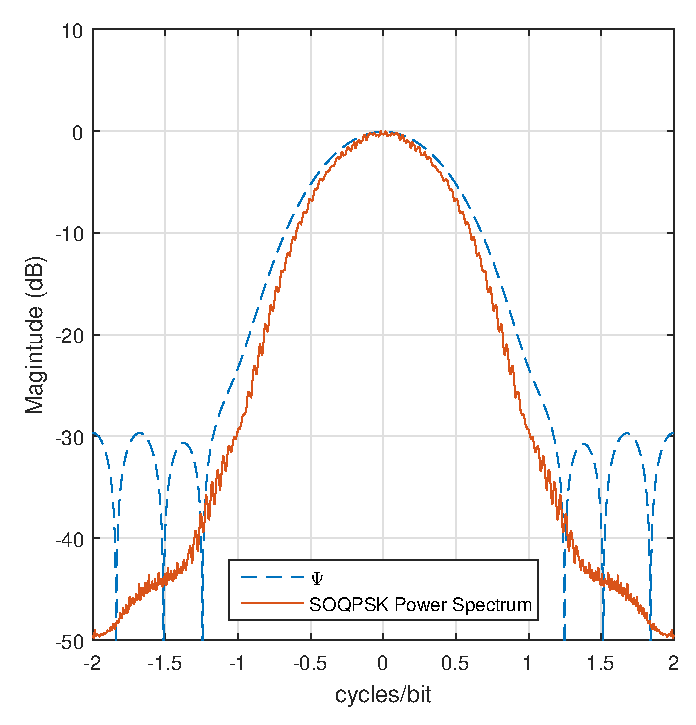
\includegraphics[width=5in]{figures/eq_equations/FDE2_spectrum_PSI.eps}
	\caption{SOQPSK-TG power spectral density.}
	\label{fig:SOQPSK_spectrum}
\end{figure}
